\documentclass[ngerman,hyperref={pdfpagelabels=false}]{beamer}

% -----------------------------------------------------------------------------

\graphicspath{{images/}}

% -----------------------------------------------------------------------------

\usetheme{KIT}

\setbeamercovered{transparent}
%\setbeamertemplate{enumerate items}[ball]

\newenvironment<>{KITtestblock}[2][]
{\begin{KITcolblock}<#1>{#2}{KITblack15}{KITblack50}}
{\end{KITcolblock}}

\usepackage[ngerman,english]{babel}
\usepackage[utf8]{inputenc}
\usepackage[TS1,T1]{fontenc}
\usepackage{array}
\usepackage{multicol}
\usepackage[absolute,overlay]{textpos}
\usepackage{beamerKITdefs}

\pdfpageattr {/Group << /S /Transparency /I true /CS /DeviceRGB>>}	%required to prevent color shifting with transparent images


\title{Algorithmen I - Tutorium 6}
\subtitle{Sebastian Schmidt -- \textit{isibboi@gmail.com}}

\author[Sebastian Schmidt]{Sebastian Schmidt}
\institute{Arbeitsgruppe Kryptographie und Sicherheit}

\TitleImage[width=\titleimagewd,height=\titleimageht]{titel}

\KITinstitute{Arbeitsgruppe Kryptographie und Sicherheit}
\KITfaculty{Fakult\"at f\"ur Informatik}

% -----------------------------------------------------------------------------

\begin{document}
\setlength\textheight{7cm} %required for correct vertical alignment, if [t] is not used as documentclass parameter


% title frame
\begin{frame}
  \maketitle
\end{frame}

\begin{frame}{Quicksort}
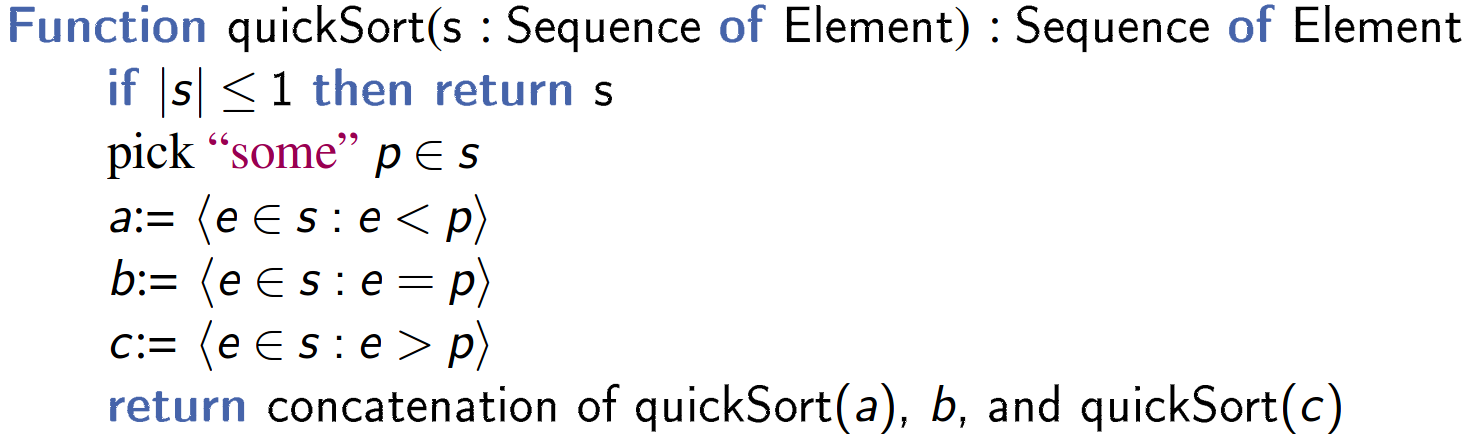
\includegraphics[width=\textwidth]{qsort_theory}

\only<1>{Beispiel: 5, 1, 0, 2, 4, 3, 6

Pivotwahl: Rechts}

\only<2>{Was ist eine Worst-Case-Eingabe, wenn als Pivot immer das rechte Element gewählt wird?}

\only<4>{Was ist eine Best-Case-Eingabe mit sieben Elementen, wenn als Pivot immer das rechte Element gewählt wird?}

\only<3>{Wie muss man das Pivot wählen, um eine aufsteigend sortierte Folge schnell zu sortieren?}

\only<4>{Wie wählt man das perfekte Pivot?

Ist das praktikabel?}

\only<5>{Welche Pivotwahl-Heuristik würdet ihr wählen, wenn ihr Quicksort implementieren müsstet?}
\end{frame}

% std::sort erklären?

\end{document}
